%%
%% @filename TD5.tex
%% @date jeu. 17 déc. 2020 11:05:17 CET
%% @author Guillaume Fornes <guillaume.fornes@enseirb-matmeca.fr>
%%
\documentclass[a4paper]{article}

\usepackage[utf8]{inputenc}
\usepackage[french]{babel} 

% Figures
\usepackage{graphicx}
\graphicspath{{./img/}}

% Math
\usepackage{amsmath, amssymb}
\newtheorem{defi}{Définition}

% Algortihmes
\usepackage[vlined,lined,linesnumbered,boxed,french]{algorithm2e}
\DeclareMathOperator*{\argmin}{argmin}
\DeclareMathOperator{\myfunc}{myfunc}
\DeclareMathOperator*{\sign}{sign}
\DeclareMathOperator*{\imwh}{width}
\DeclareMathOperator*{\imht}{height}

% Extra
\usepackage[left=3cm,right=3cm,top=2cm,bottom=2cm]{geometry}
\usepackage{url}
\setcounter{totalnumber}{8}

\begin{document}
\part*{Spécificité terminaison et correction de programme}
\section*{Exercice 1}
\begin{figure}[!h]
  \centering
  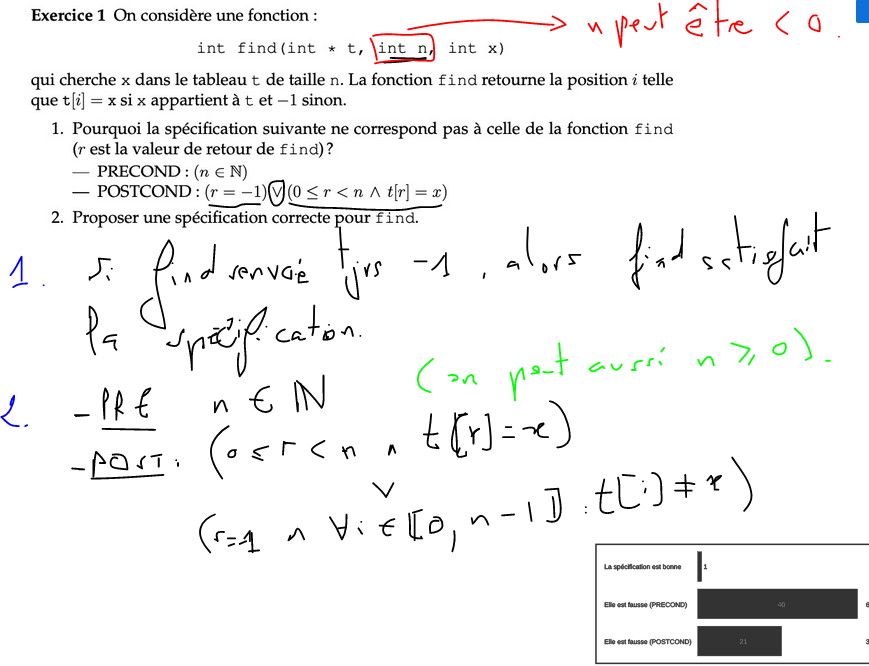
\includegraphics[scale=0.60]{ex1_td5}
\end{figure}
\section*{Exercice 2}
PRECOND :\\

POSTCOND:\\
malheureusement disparu !

\clearpage
\section*{Exercice 3}

\begin{figure}[!h]
  \centering
  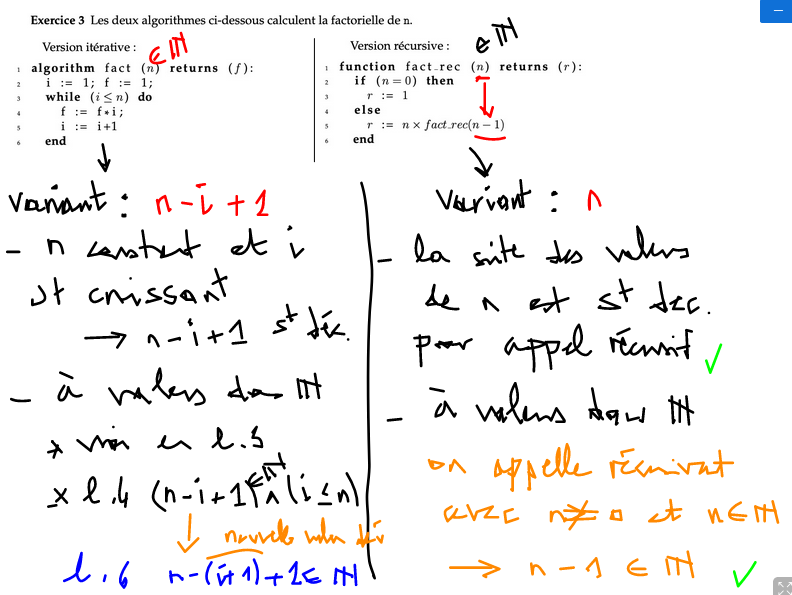
\includegraphics[scale=0.65]{ex3_td5}
\end{figure}
\begin{figure}[!h]
  \centering
  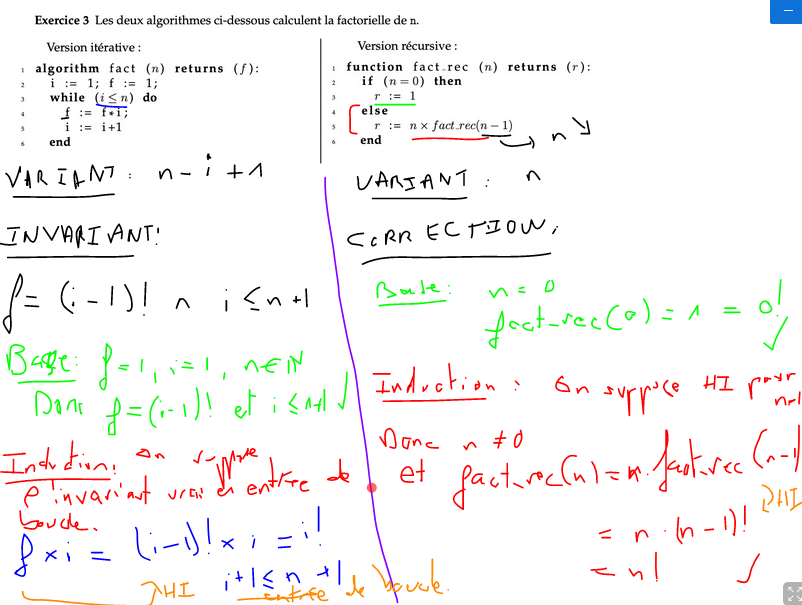
\includegraphics[scale=0.65]{ex3bis_td5}
\end{figure}
\begin{figure}[!h]
  \centering
  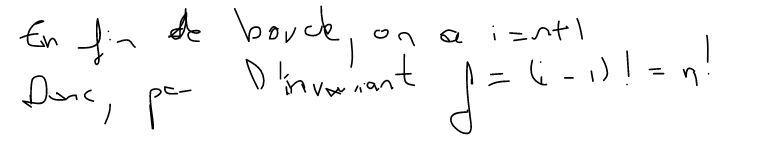
\includegraphics[scale=0.65]{ex3ter_td5}
\end{figure}


\clearpage
\section*{Exercice 4}

\begin{figure}[!h]
  \centering
  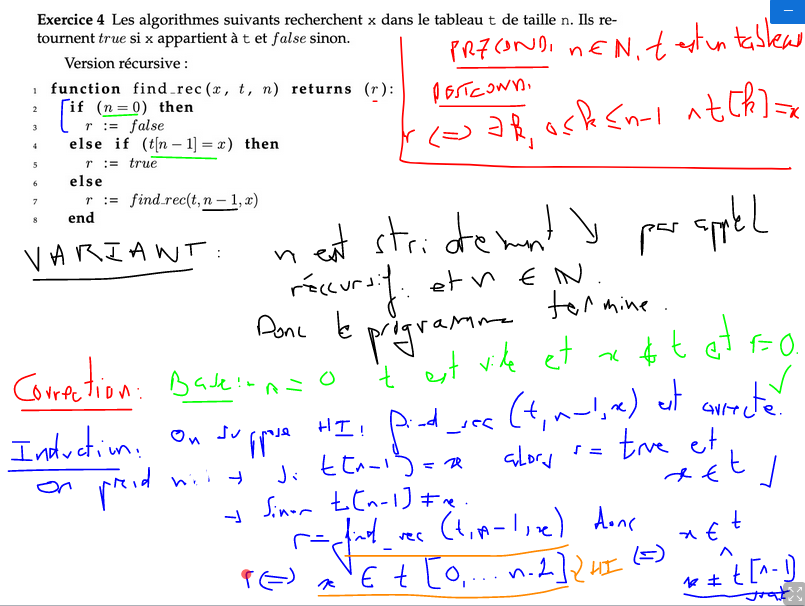
\includegraphics[scale=0.5]{ex4_td5}
\end{figure}
\begin{figure}[!h]
  \centering
  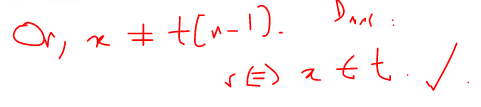
\includegraphics[scale=0.5]{ex4bis_td5}
\end{figure}
\begin{figure}[!h]
  \centering
  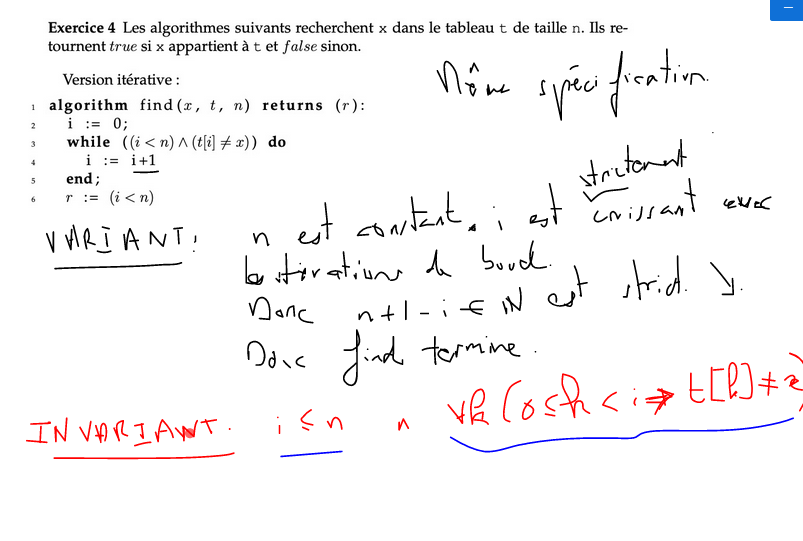
\includegraphics[scale=0.5]{ex4ter_td5}
\end{figure}
\begin{figure}[!h]
  \centering
  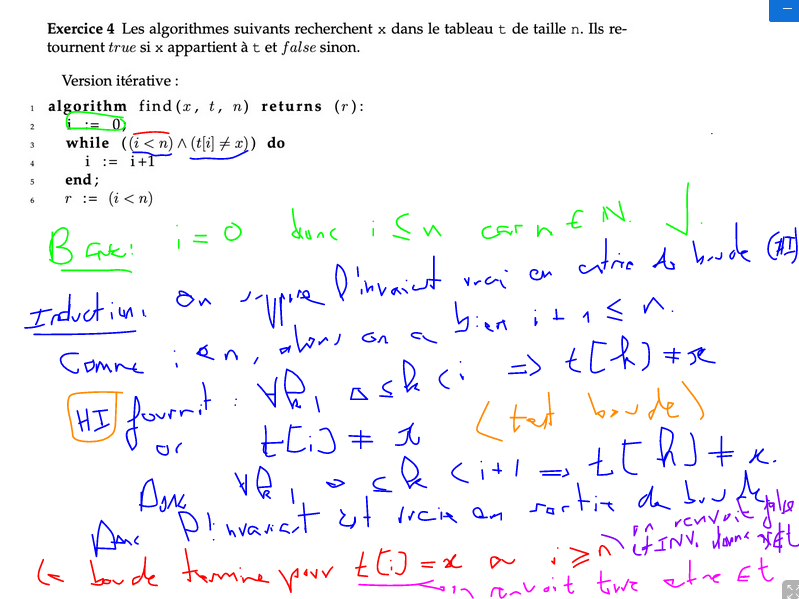
\includegraphics[scale=0.5]{ex44_td5}
\end{figure}


\clearpage
\section*{Exercice 5}
\begin{figure}
  \centering
  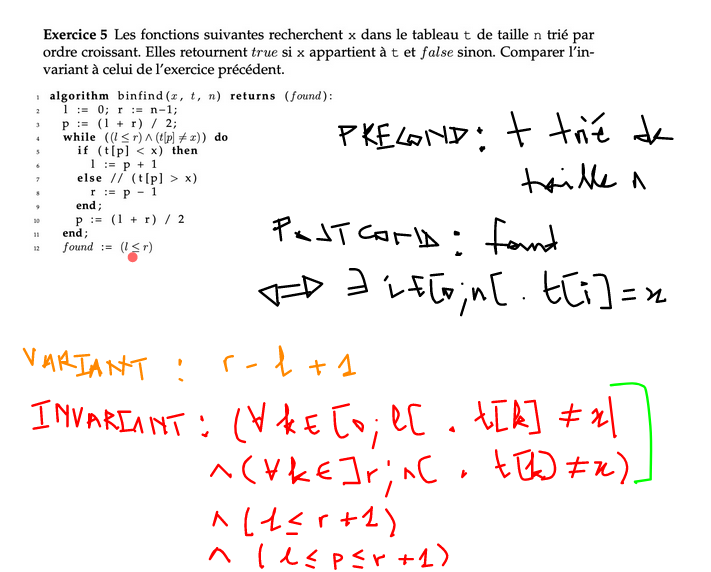
\includegraphics[scale=0.5]{ex5_td5}
\end{figure}
\clearpage
\section*{Exercice 6}
\underline{Terminaison} variant l\\
\begin{itemize}
  \item strictement décroissante par appel récursif / validé car tl est une sous liste de l\\
  \item à valeur dans un ensemble bien fondé / validé car $tl <_{L}hd::tl$ $\forall hd, tl$\\
    est bien fondé sur le type $List$ (théorème 7.3)\\
\end{itemize}
\underline{Correction}
\begin{itemize}
  \item PRECOND : $l\in List$
  \item POSTCOND : $is\_{sorted}(l) \iff (\forall i\in [0;|l|[.l_{i}\leq l_{i+1}) $\\
\end{itemize}
\underline{Cas de base :}\\
si $l=[  ] \rightarrow is\_sorted(l)=true$ validé !\\
si $l=hd::[] \rightarrow is\_{sorted}(l)=true $ validé !\\
\underline{Induction :} On suppose l'appel récursif correct, (HI, la ligne 5)\\
$hd::\underbrace{hd_{2}::tl_{2}}$ il faut que tl trié $\leftarrow bon par HI \implies is\_{sorted(l)}$ correct\\
.\hspace{10mm} tl
\begin{figure}[!h]
  \centering
  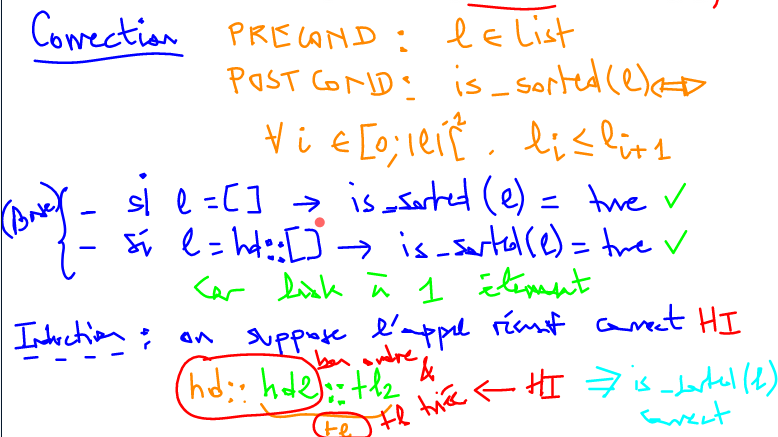
\includegraphics[scale=0.5]{td5_ex6}
\end{figure}
\end{document}
